\section{References \& Further Reading}

\begin{frame}
\frametitle{Essential References}

\begin{mathbox}{Foundational Texts}
\begin{itemize}
    \item \textbf{Real-Time Rendering, 4th Edition} \\
          Akenine-Möller, Haines, Hoffman, et al. (2018)
    \item \textbf{Computer Graphics: Principles and Practice, 3rd Edition} \\
          Hughes, van Dam, McGuire, et al. (2013)
    \item \textbf{Fundamentals of Computer Graphics, 5th Edition} \\
          Marschner \& Shirley (2021)
\end{itemize}
\end{mathbox}

\begin{conceptbox}{GPU Architecture \& Programming}
\begin{itemize}
    \item \textbf{GPU Gems Series} - NVIDIA (Free online)
    \item \textbf{GPU Pro Series} - Annual collection of advanced techniques
    \item \textbf{Graphics Programming and Shaders} - Bailey \& Cunningham
    \item \textbf{OpenGL Programming Guide} - The Khronos Group
\end{itemize}
\end{conceptbox}

\end{frame}

\begin{frame}
\frametitle{Online Resources}

\begin{conceptbox}{Documentation \& Specifications}
\begin{itemize}
    \item \textbf{OpenGL Specification}: \url{https://www.opengl.org/}
    \item \textbf{Vulkan Specification}: \url{https://www.vulkan.org/}
    \item \textbf{DirectX Documentation}: \url{https://docs.microsoft.com/en-us/windows/win32/direct3d}
    \item \textbf{WebGL Specification}: \url{https://www.khronos.org/webgl/}
\end{itemize}
\end{conceptbox}

\begin{mathbox}{Learning Resources}
\begin{itemize}
    \item \textbf{LearnOpenGL}: \url{https://learnopengl.com/}
    \item \textbf{Scratchapixel}: \url{https://www.scratchapixel.com/}
    \item \textbf{Inigo Quilez}: \url{https://iquilezles.org/}
    \item \textbf{Simon's Graphics Blog}: \url{https://simonschreibt.de/}
\end{itemize}
\end{conceptbox}

\end{frame}

\begin{frame}
\frametitle{Academic Papers \& Research}

\begin{mathbox}{Foundational Papers}
\begin{itemize}
    \item \textbf{A Hidden-Surface Algorithm with Anti-Aliasing} \\
          Catmull (1974) - Z-buffer algorithm
    \item \textbf{The A-buffer, an antialiased hidden surface method} \\
          Carpenter (1984) - Anti-aliasing techniques
    \item \textbf{Reality Engine Graphics} \\
          Akeley (1993) - Hardware rasterization
    \item \textbf{WireGL: A Scalable Graphics System for Clusters} \\
          Humphreys et al. (2001) - Distributed rendering
\end{itemize}
\end{mathbox}

\begin{conceptbox}{Modern Techniques}
\begin{itemize}
    \item \textbf{Deferred Shading} - Saito \& Takahashi (1990)
    \item \textbf{Cascaded Shadow Maps} - Zhang et al. (2006)
    \item \textbf{Screen Space Ambient Occlusion} - Mittring (2007)
    \item \textbf{Temporal Anti-Aliasing} - Yang et al. (2009)
\end{itemize}
\end{conceptbox}

\end{frame}

\begin{frame}
\frametitle{Industry Resources}

\begin{conceptbox}{Hardware Vendor Resources}
\begin{itemize}
    \item \textbf{NVIDIA Developer}: \url{https://developer.nvidia.com/}
          \begin{itemize}
              \item CUDA Programming Guide
              \item RTX Developer Resources
              \item Nsight Graphics Documentation
          \end{itemize}
    \item \textbf{AMD Developer Central}: \url{https://gpuopen.com/}
          \begin{itemize}
              \item Radeon GPU Analyzer
              \item FidelityFX SDK
              \item Performance Optimization Guides
          \end{itemize}
    \item \textbf{Intel Graphics Developers}: \url{https://www.intel.com/content/www/us/en/developer/}
          \begin{itemize}
              \item Graphics Performance Analyzers
              \item oneAPI Toolkit
          \end{itemize}
\end{itemize}
\end{conceptbox}

\end{frame}

\begin{frame}
\frametitle{Tools \& Software}

\begin{mathbox}{Graphics Debugging \& Profiling}
\begin{itemize}
    \item \textbf{RenderDoc}: Free, open-source graphics debugger
    \item \textbf{NVIDIA Nsight Graphics}: Advanced GPU debugging
    \item \textbf{AMD Radeon GPU Profiler}: Performance analysis
    \item \textbf{Intel Graphics Performance Analyzers}: Cross-platform profiling
    \item \textbf{Xcode GPU Debugger}: Metal debugging on macOS/iOS
\end{itemize}
\end{mathbox}

\begin{conceptbox}{Development Frameworks}
\begin{itemize}
    \item \textbf{OpenGL}: Cross-platform graphics API
    \item \textbf{Vulkan}: Low-level, high-performance API
    \item \textbf{Direct3D}: Microsoft's graphics API
    \item \textbf{Metal}: Apple's graphics and compute API
    \item \textbf{WebGL/WebGPU}: Browser-based graphics
\end{itemize}
\end{conceptbox}

\end{frame}

\begin{frame}
\frametitle{Conferences \& Communities}

\begin{conceptbox}{Major Conferences}
\begin{itemize}
    \item \textbf{SIGGRAPH}: Premier computer graphics conference
    \item \textbf{GDC}: Game Developers Conference
    \item \textbf{High Performance Graphics (HPG)}: Academic rendering research
    \item \textbf{Eurographics}: European computer graphics conference
    \item \textbf{I3D}: Interactive 3D Graphics and Games
\end{itemize}
\end{conceptbox}

\begin{mathbox}{Online Communities}
\begin{itemize}
    \item \textbf{Graphics Programming Discord/Reddit}: Active communities
    \item \textbf{Shadertoy}: \url{https://www.shadertoy.com/} - Shader playground
    \item \textbf{GitHub}: Open-source graphics projects and demos
    \item \textbf{Stack Overflow}: Q\&A for specific technical issues
    \item \textbf{Graphics Programming Weekly}: Curated news and resources
\end{itemize}
\end{mathbox}

\end{frame}

\begin{frame}
\frametitle{Recommended Learning Path}

\begin{center}
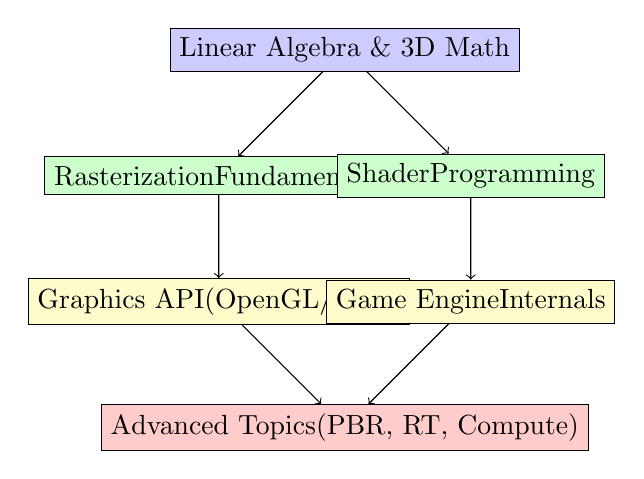
\begin{tikzpicture}[scale=0.8]
    % Learning path flowchart
    \node[draw, rectangle, fill=blue!20] (basics) at (0,4) {Linear Algebra \& 3D Math};
    
    \node[draw, rectangle, fill=green!20] (raster) at (-2,2) {Rasterization \\ Fundamentals};
    \node[draw, rectangle, fill=green!20] (shaders) at (2,2) {Shader \\ Programming};
    
    \node[draw, rectangle, fill=yellow!20] (api) at (-2,0) {Graphics API \\ (OpenGL/D3D)};
    \node[draw, rectangle, fill=yellow!20] (engine) at (2,0) {Game Engine \\ Internals};
    
    \node[draw, rectangle, fill=red!20] (advanced) at (0,-2) {Advanced Topics \\ (PBR, RT, Compute)};
    
    \draw[->] (basics) -- (raster);
    \draw[->] (basics) -- (shaders);
    \draw[->] (raster) -- (api);
    \draw[->] (shaders) -- (engine);
    \draw[->] (api) -- (advanced);
    \draw[->] (engine) -- (advanced);
\end{tikzpicture}
\end{center}

\begin{conceptbox}{Practice Projects}
\begin{enumerate}
    \item Software rasterizer implementation
    \item Simple OpenGL/Vulkan renderer
    \item Deferred rendering pipeline
    \item Shadow mapping techniques
    \item Post-processing effects
\end{enumerate}
\end{conceptbox}

\end{frame}
